\section{IMPLEMENTATION} 
\subsection{Overview} The method used for course optimization is Maximum Bipartite Matching. The code has been implemented in Python language, using the NetworkX library and Enumerating Maximum Matching Algorithm (EMMA). By applying necessary constraints to eliminate undesired matchings, we obtain and display the acceptable allocations, rank ordered by score which is based on preference order given by professors.
\subsection{Detailed Explanation} The optimization problem at hand contains 3 categories of professors, accepting 0.5 (1 unit), 1 (2 units) and 1.5 (3 units) courses respectively. [Note: According to the problem statement, category 3 professors can accept either 1 or 1.5 course (either 2 or 3 units).] There are also 2 types of courses, CDCs and Electives, each having 2 units. This is shown in the following table:-
\begin{table}[h]
		\centering
		\Medium{
			\begin{tabular}{>{\bfseries}lc>{\bfseries}r}
				1. Professor & 0.5 Course (Category 1) & 1 Unit\\ & 1.0 Course (Category 2) & 2 Units\\ & 1.5 Course (Category 3) & 3 Units\\ \\2. Course & CDC & 2 Units\\& Elective & 2 Units\\
		\end{tabular}}
	\end{table}
\\
The approach that we take to solve this problem is by finding bipartite graph matchings between 2 sets of nodes where one set of nodes represents professors while the other set represents courses. Since each professor can teach multiple courses, and each course can be taught by multiple professors, we have a many-many biparite matching problem. Tackling this problem in its present state is undesirably complex. Therefore, we convert this to a one-one matching problem by splitting individual professors and courses into nodes such that each unit represents a single node. This assignment of nodes is as follows:-
\begin{table}[h]
		\centering
		\Medium{
			\begin{tabular}{>{\bfseries}lc>{\bfseries}r}
				1. Professor & & 0.5 Course(Category 1) & & 1 Unit & & 1 Node\\ & & 1.0 Course(Category 2) & & 2 Units & & 2 Nodes\\ & & 1.5 Course(Category 3) & & 3 Units & & 3 Nodes\\ \\2. Course & & CDC & & 2 Units & & 2 Nodes\\& & Elective & & 2 Units & & 2 Nodes\\
		\end{tabular}}
	\end{table}
\\ \\ \\ 
Now that we have converted our problem into a one-one bipartite matching problem format, we proceed in the following fashion:
\begin{enumerate}
\item Generating all possible one-one maximum bipartite matchings using Enumerating Maximum Matchings Algorithm (EMMA).
\paragraph{} A Maximum Bipartite Matching is a matching in a bipartite graph that contains the maximum number of edges and where no more edges can be added.\\
EMMA is an algorithm in the paper ``Algorithms for Enumerating All Perfect, Maximum and Maximal Matchings in Bipartite Graphs" by Takeaki Uno. According to Theorem 2 in this paper, time complexity of the alogrithm is \(O(mn^{1/2} +nN_m)\) and space complexity is \(O(m)\), where $N_m$ is the number of maximum matchings in G. We use a python implementation of this algorithm by Guangzhi XU which makes use of NetworkX and NumPy modules.

\item  We weed out undesirable matchings that do not satisfy the following constraints:
\begin{enumerate}
\item All nodes of professors of categories 1 and 2 should be assigned an edge. 
\item For all category 3 professors, 2 or 3 nodes should be assigned an edge.
\item Both nodes of all CDCs should be assigned an edge.
\item For electives, either both or no nodes should be assigned an edge.\\
We need to check for certain eligible matchings which are not maximum but whose maximum version is eliminated due to this constraint. Such matchings occur because of some peculiar elective-professor edges. If an elective has only one unit assigned to a category 3 professor, whose other 2 nodes are assigned to a single distinct course, or, separately assigned to two completely satisfied courses, then the edge joining the professor to the elective can be safely removed so as to incorporate the rest of the matching into the list of satisfactory matchings. We do this for all such electives to get the final desirable matching.
\end{enumerate}
\begin{figure}[h]
    \centering
    \caption{This figure demonstrates the edges to be removed.}
    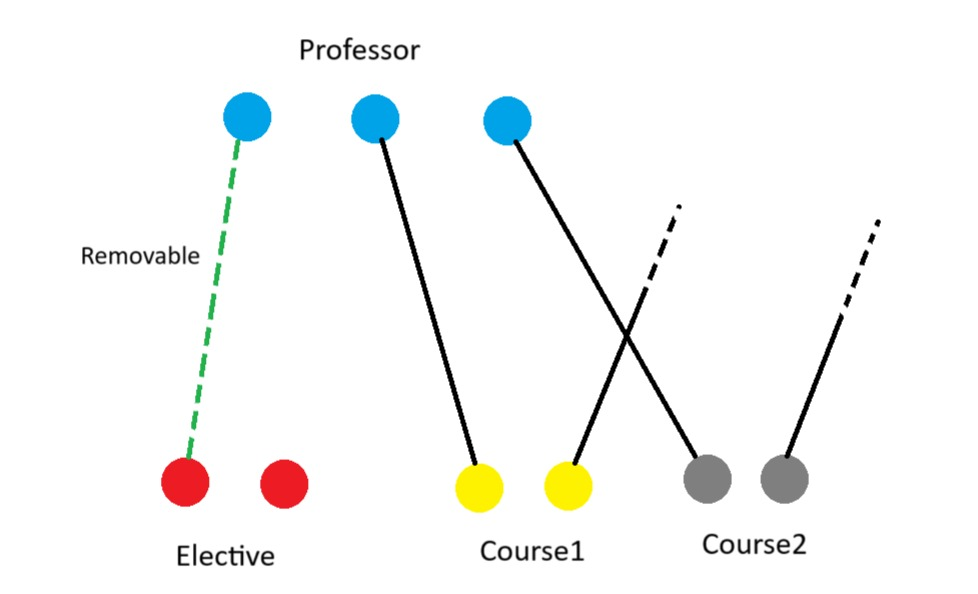
\includegraphics[width=0.5\textwidth]{images/Remove.jpeg}
\end{figure}\\

\item Now that we have matchings that satisfy the aforementioned constraints, we convert them back into our original format of Professors and Courses.
\paragraph{} We do this to eliminate all the repetitions caused by intra-matching within the nodes of the same professor-course pairs.
\item  We now assign Satisfaction Scores to each matching in accordance with the priority orders of Courses in the Professors' Preferences.
\paragraph{} For each edge in the matching we add  \(Max\_Points - k\)  to get the Satisfaction Score of that matching, where k is the priority index of the course in the professor's preference order for respective professor-course pairs.  \(Max\_Points\)  is the total number of courses. We add this term to ensure that the edge score always remains positive. Rank-ordering of desired matchings is performed based on the descending order of Satisfaction Scores. Matchings with higher Satisfaction Scores are preferred.
\end{enumerate}
Thus, we present a list of all possible allocations of courses to professors, satisfying all constraints and maximizing preferences, in decreasing order of desirability.
\newpage

